\section{Quantum Field Theory}
\subsection{The Weak Interaction}
\subsection{Quantum Electrodynamics}
\subsection{Quantum Chromodynamics}

\section{The Standard Model}

The Standard Model (SM)\cite{SM1} is a theory that stems from the unification of the electroweak theory (EWT)\cite{EWT}, which unifies the weak interaction and quantum electrodynamics (QED) theories, and quantum chromodynamics (QCD)\cite{QCD}, which together describes the electromagnetic, weak and strong interactions and has been able to correctly predict the existence and interactions of all currently discovered particles. It was developed throughout the latter half of the 20th century, as a collaborative effort of scientists around the world. According to this theory all matter is composed of the three different groups of particles described in the SM: leptons, quarks and force mediators. Alternatively, these particles can also be categorized according to their quantum spin number. Particles with whole integer spin like the mediators are called bosons, while particles with spin one half, like leptons and quarks, are called fermions. Accounting for particles of different charge, color and their antimatter partners, there is a total of 61 particles in the SM: 48 fermions (36 quarks and 12 leptons) and 13 bosons. The Higgs boson\cite{Higgs1} was the only missing piece of the SM and, nearly 50 years after initially proposed, it was finally discovered at the LHC in 2012 \cite{Higgs,Higgs2}. The Higgs boson is a particle corresponding to the Higgs field which, according to the SM, gives mass to all the fundamental particles.

\begin{comment} %
\begin{figure}[tb]
\begin{center}
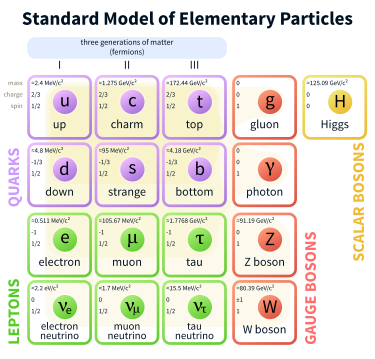
\includegraphics[width=0.5\textwidth]{SM.png} 
\caption{Schematic representation of the Standard Model particles. Shown are the three generations of matter (formed by fermions), the gauge bosons and the Higgs boson.}
\label{SM.png} 
%\hspace{4em}
\end{center}
\end{figure}
\end{comment} %

\subsection{SM particles}
\subsection{The Higgs Boson}
\section{Physics Beyond the Standard Model}
\subsection{Supersymmetry}
\subsection{Other BSM Studies}
